\section{Data}
\label{sec:data}

\subsection{Data source and selection}
Data is from the Swedish Labour Force Survey (LFS) and covers the period 1987-2012 \citep{AKU2012}. During this period the survey samples 17 000-29 500 individuals each month. The survey began already in 1961, but micro data is only available for 1987 and onwards. The survey samples individuals from a register containing the entire population in Sweden (RTB). Up to 2001 the sample includes all ages 16-64, but in 2001 the age interval was expanded to 15-74. For consistency, we will however confine our sample to ages 16-64. 

The survey sample is rotating (Figure \ref{tab:rot_panel}). Specifically, a participating individual is interviewed about his or her employment status at a given week every third month during two years. In each month 8 groups of individuals are interviewed. 7 of these 8 groups have been interviewed previously, while 1 group is being interviewed for the first time. Consequently, one group is rotating out(in) of the sample at each point in time.

The surveyed population is divided into the following categories (i) employed, (ii) unemployed or (iii) outside the labour force (Figure \ref{fig:LFS_clas}). The individual is characterised as \textit{employed} if she was working at least one hour during the reference week as (a) self-employed (including helping spouse) (c) on a permanent contract (\textit{tillsvidereanstallning}) or (d) on a time-limited contract. An individual who has a job but was absent work due to illness, leave, vacation, military service, a conflict or similar is also counted as employed. So is an individual in a labour market program, if she receive some enumeration from the employer. The individual is characterised as \textit{unemployed} if she is not employed, but has been applying for work within the last four weeks and is able to start work within the reference week or the two following weeks. An individual is also characterised as unemployed if the person is set to start a job within the next three months, provided that the individual would be ready to start already in the reference week or during the following two weeks. Finally, an individual is characterised as \emph{outside the labor force} if she is not covered by the definitions above. This includes individuals who would and could be able to work, but who did not actively seek jobs (\textit{latent unemployment}). 

In 2007 the treatment of students was altered, so as to comply with ILO definitions. Up to this point full-time students who also applied for jobs were counted as outside the labour force. But from 2007 these are counted as unemployed. For the age group 16-64, which we confine our sample to, this definition is applied through the entire sample. 

We clean and seasonally correct data before conducting our analysis. Data is very thin with only around 200 observations in the period 2004M10-2004M12 [TDB: Ask SCB why]. In order avoid having our variation driven by thin data collection, we interpolate all transition rates and stock shares during this period. We correct the diagonal in the interpolated transition matrix to make sure it sums to one. We also seasonally correct transition and stock rates in order to abstract from high frequency variation. Specifically, we apply a 12 month centered moving average correction such that the observed data at time $t$ is a weighted average of data in the interval $[t-5, t+6]$ [TBD: Should we do 13 months?]. 

\subsection{Labor market stocks and flows}
Figure \ref{fig:LFS_states} shows the stock of employed, unemployed and inactive in Sweden since 1987. The period covers approx. two business cycles as unemployment troughs and peaks in 1990/2008 and 1996/2001, respectively. The overall employment rate is falling approximately 10 percentage points through the period (from 82 to 70 percent), with inactivity rising similarly. The change in the overall employment rate covers diverse changes for permanent and temporary employment, however. While the share of the population on permanent employment is down 10 percentage points, the share on temporary employment has risen slightly. Consequently, the share of workers on temporary contracts has increased from 20 to 24 percent.

Figure \ref{fig:hazard_rates}-\ref{fig:log_hazard_rates} show the flows moving between the four groups computed as monthly hazard rates (see Section \eqref{sec:est_flow_matrices} for computation method). From these figures two trends are visible. First, all the flow rates into permanent and temporary employment have decreased. Second, the probability of flowing from employment into unemployment has increased. There is no clear trend in the hazard rates for movements into inactivity. 

TBD: Describe how hazards are computed

TBD: Describe how we handle Seasonality

\subsection{Cyclicality of flows}

Table \ref{tab:flow_cyc} illustrates the sensitivity of labour market flows with respect to the business cycle. We gauge this by regressing the relevant hazard rate (logged) on the the unemployment rate and a linear trend. Table \ref{tab:flow_cyc} reports the coefficient on the unemployment rate from this regression. A positive (negative) value in Table \ref{tab:flow_cyc} indicates that the correlation between the relevant flow and unemployment is positive (negative). Consequently, a negative (positive) value indicates that the flow is pro-cyclical (counter-cyclical). Thus, from Table \ref{tab:flow_cyc} we see that all flows into permanent and temporary employment are pro-cyclical, while all flows into unemployment are countercyclical. The flow from permanent employment to inactivity is from regular (temporary) employment is pro-cyclical (a-cyclical), while the flow from temporary employment to inactivity is counter-cyclical. 

\begin{table}[h]
	\caption{Illustration of the rotating panel structure}
	\label{tab:rot_panel}
	\begin{tabularx}{\linewidth}{cXccccccccc}
	\toprule[1pt] 
	 && Group 1 & Group 2 & Group 3 & Group 4 & Group 5 & Group 6  & Group 7 & Group 8 \\ \hline 
Month 0 && $\mathbf{G_{0}}$ & $G_{-3}$ & $G_{-6}$ & $G_{-9}$ & $G_{-12}$ & $G_{-15}$ & $G_{-18}$ & $G_{-21}$ \\
Month 1 && $G_{1}$ & $G_{-2}$ & $G_{-5}$ & $G_{-8}$ & $G_{-11}$ & $G_{-14}$ & $G_{-17}$ & $G_{-20}$ \\
Month 2 && $G_{2}$ & $G_{-1}$ & $G_{-4}$ & $G_{-7}$ & $G_{-10}$ & $G_{-13}$ & $G_{-15}$ & $G_{-19}$ \\ 
Month 3 && $G_{3}$ & $\mathbf{G_{0}}$ & $G_{-3}$ & $G_{-6}$ & $G_{-9}$ & $G_{-12}$ & $G_{-14}$ & $G_{-18}$ \\
Month 4 && $G_{4}$ & $G_{1}$ & $G_{-2}$ & $G_{-5}$ & $G_{-8}$ & $G_{-11}$ & $G_{-14}$ & $G_{-17}$ \\  
Month 5 && $G_{5}$ & $G_{2}$ & $G_{-1}$ & $G_{-4}$ & $G_{-7}$ & $G_{-10}$ & $G_{-13}$ & $G_{-16}$ \\ 
Month 6 && $G_{6}$ & $G_{2}$ & $\mathbf{G_{0}}$ & $G_{-3}$ & $G_{-6}$ & $G_{-9}$ & $G_{-12}$ & $G_{-16}$ \\ 
Month 7 && $G_{7}$ & $G_{4}$ & $G_{1}$ & $G_{-2}$ & $G_{-5}$ & $G_{-8}$ & $G_{-11}$ & $Gdv_{-14}$ \\ 
Month 8 && $G_{8}$ & $G_{5}$ & $G_{2}$ & $G_{-1}$ & $G_{-4}$ & $G_{-7}$ & $G_{-10}$ & $G_{-13}$ \\ 
Month 9 && $G_{9}$ & $G_{6}$ & $G_{3}$ & $\mathbf{G_{0}}$ & $G_{-3}$ & $G_{-6}$ & $G_{-9}$ & $G_{-12}$ \\ 
Month 10 && $G_{10}$ & $G_{7}$ & $G_{4}$ & $G_{1}$ & $G_{-2}$ & $G_{-5}$ & $G_{-8}$ & $G_{-11}$ \\ 
Month 11 && $G_{11}$ & $G_{8}$ & $G_{7}$ & $G_{4}$ & $G_{1}$ & $G_{-2}$ & $G_{-5}$ & $G_{-8}$ \\
Month 12 && $G_{12}$ & $G_{9}$ & $G_{6}$ & $G_{3}$ & $\mathbf{G_{0}}$ & $G_{-3}$ & $G_{-6}$ & $G_{-9}$ \\  
	\bottomrule[1pt]
	\end{tabularx}
	\begin{minipage}{\linewidth}
		\footnotesize{Notes: $G_n$ is group of individuals who entered the survey in month $n$. Each group is surveyed with an interval of 3 months. In each month 7/8 of the sample has been surveyed before. 1/8 of the sample is surveyed for the first time.}
	\end{minipage}
\end{table}	

\begin{figure}
	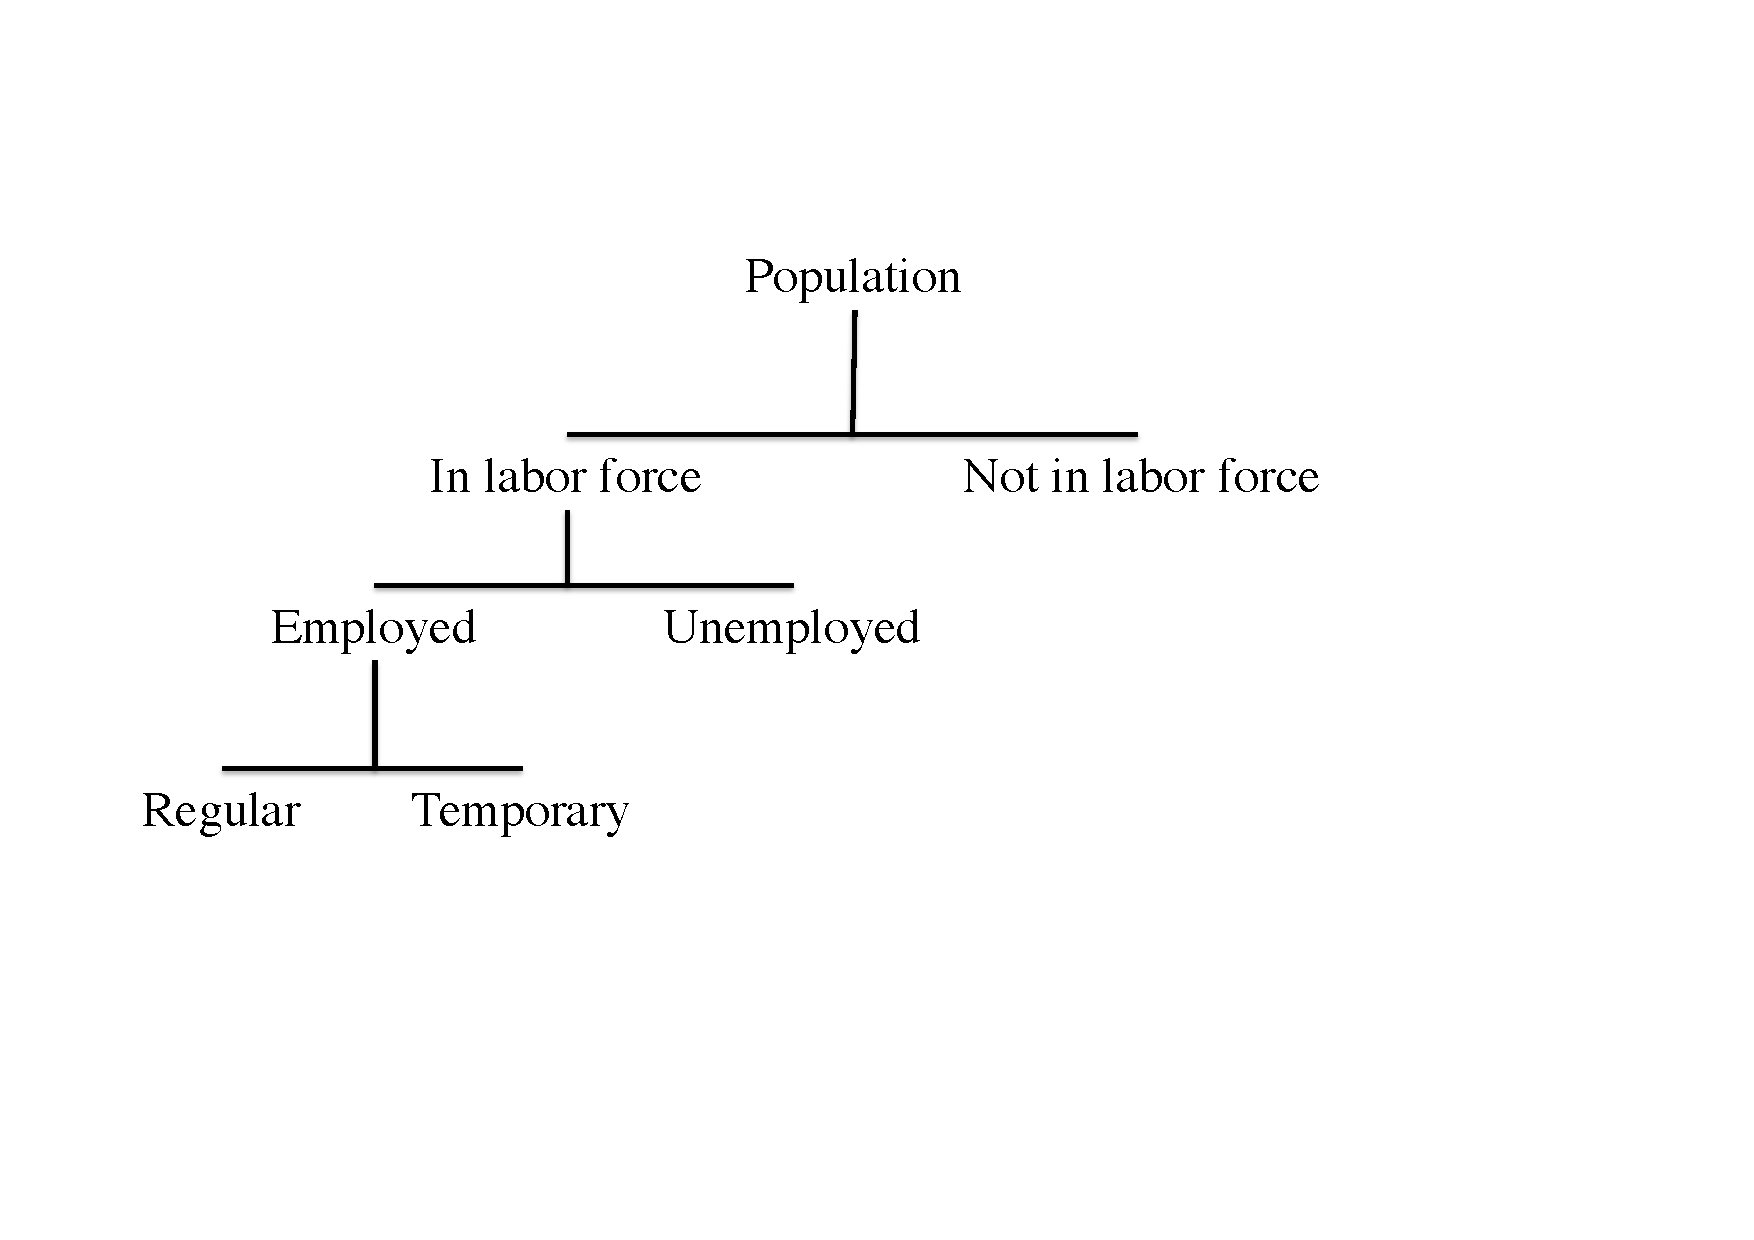
\includegraphics[scale=0.65, trim=2cm 6cm 7cm 4cm, clip]{Figures/population}
	\caption{Basic classification of population in labor force survey}
	\label{fig:LFS_clas}
\end{figure}

\begin{landscape}
\begin{figure}
\centering
	\includegraphics[scale=0.8, trim=2cm 2cm 0cm 1cm, clip]{../../Programs/Figures/fig_descriptive_states.pdf}
	\caption{Labour market stocks across time}
	\label{fig:LFS_states}
\end{figure}
\end{landscape}

%\begin{landscape}
%\begin{figure}
%\centering
	%\includegraphics[scale=0.8, trim=2cm 2cm 0cm 1cm, clip]{../../Programs/Figures/fig_gross_flows_prob.pdf}
	%\caption{Gross flows between labour market states}
	%\label{fig:LFS_states}
%\end{figure}
%\end{landscape}

\begin{landscape}
\begin{figure}
\centering
	\includegraphics[scale=0.8, trim=2cm 2cm 0cm 1cm, clip]{../../Programs/Figures/fig_hazard_rates.pdf}
	\caption{Hazard rates for transition across labour market states}
	\label{fig:hazard_rates}
\end{figure}
\end{landscape}

\begin{landscape}
\begin{figure}
\centering
	\includegraphics[scale=0.8, trim=2cm 2cm 0cm 1cm, clip]{../../Programs/Figures/fig_log_hazard_rates.pdf}
	\caption{Hazard rates for transition across labour market states, logged}
	\label{fig:log_hazard_rates}
\end{figure}
\end{landscape}

\begin{table}[h]
	\caption{Cyclical variation in hazard rates}
	\label{tab:flow_cyc}
	\begin{tabularx}{\linewidth}{cXccccccccc}
	\toprule[1pt] 
	             && Permanent emp. & Temporary emp.     & Unemployment   & Inactivity  \\ \hline 
Permanent emp. &&                &  $-6.8117^{***}$   & $ 8.0218^{***}$ & -0.9282$^{***}$ \\
Temporary emp. &&  $-6.6049^{***}$     &                    &$11.3282^{***}$        &$-0.0401$ \\
Unemployment   &&  $-20.5563^{***}$     & $-12.1247^{***}$          &                &$ 3.1729^{***}$ \\ 
Inactivity   && $ -10.5943^{***}$      & $-2.9194 ^{***}$        & $18.5694^{***}$         &  \\
	\bottomrule[1pt]
	\end{tabularx}
	\begin{minipage}{\linewidth}
		\footnotesize{Notes: The reported figure is the the coefficient of the unemployment rate in a regression of the relevant hazard rate logged. Time trends are included in the regression. *(**)[***] denotes significance on 10(5)[1] pct. level. Sample period is 1987m1-2011m9.}
	\end{minipage}
\end{table}	
